\documentclass{article}
\usepackage[utf8]{inputenc}
\usepackage{natbib}
\usepackage{graphicx,physics}
\usepackage{epstopdf}
\usepackage{amsmath,amsthm,amsfonts,amssymb,mathrsfs,bm,mathtools}
\usepackage[utf8]{inputenc}
\usepackage{esvect}
\usepackage{esdiff}
\usepackage{float}
\usepackage{wrapfig}
\usepackage{systeme}
\usepackage{tikz, gensymb}
\usepackage{geometry}
\usepackage[font = footnotesize]{caption}
\usepackage{subcaption}
\usepackage{pgfplots}
	\pgfplotsset{compat = 1.9}
\usepackage{array}
\usepackage{siunitx}
\usepackage{upgreek}
\usepackage[hidelinks]{hyperref}
\graphicspath{ {./images/} }
\geometry{margin=1in}

\title{MNXB01-3.1}
\author{Anna Lena Hölldobler}
\date{November 2021}

\begin{document}

\maketitle

\section*{Goal}
The goal is to produce a function that shows a histogram of the temperatures for one day. There are supposed to be two ways to declare the function. The first option has a certain day and month as argument and the second one should take the number of a day as argument. Using the histogram, predictions can be made for the temperature at a certain day.

\section*{Method}
The first function is called tempOnDay. In the first option for the declaration, the function takes to integers as argument, the first one defining the month and the second one defining the day. A new histogram is created using the 1d histogram class of root TH1. Next the data is read in, using a while loop. The data is stored in four different lists, one list for each, year, month, day and temperature measured at noon. Then the histogram is getting filled using a for loop, running through all lines in the arrays. With if statements it gets checked, whether day and month fit to the values defined by the function arguments. When this is the case the corresponding temperature gets filled into the histogram. Last the mean value and the standard deviation are getting calculated using the functions GetMean() and GetRMS().\\\\
The second option for declaration is to define the day of a year by a number between 1 and 355. In this case the same commands as in the first case can be used, but before that the date of the day needs to be found. To do this a separate array is defined, storing the number of days for all months. Moreover, a separate count variable is defined, which is used to add the days for several month. In a for loop the number of the day is compared to the count variable, which increases by the number of days of the month in every loop. If the count value is larger than the number of the day, the date can be obtained.

\section*{Results}
Both functions obtain a plot, as it is shown in Figure \ref{fig:3.1}. Here, Karlstad and November 5th is used as an example. Furthermore, the functions provide that the mean temperature in this case is $5.34818\degree$C and the standard deviation equals $3.1245\degree$C.
\begin{figure}[H]
    \centering
    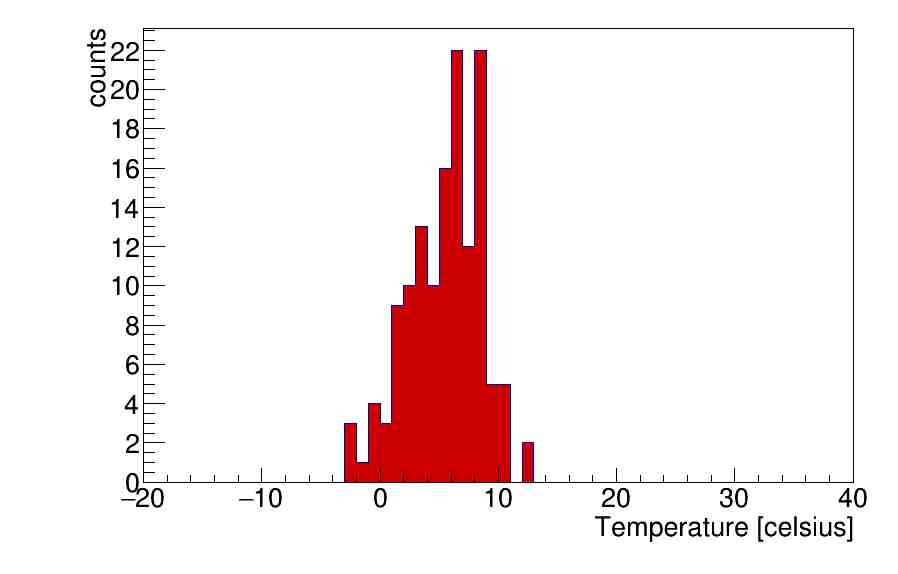
\includegraphics[scale = 0.45]{31_twoargs.jpg}
    \caption{Histogram of temperatures from Karlstad November 5th every year since 1942.}
    \label{fig:3.1}
\end{figure}

\end{document}
